\documentclass{standalone}
\usepackage{tikz}
\usetikzlibrary{patterns, positioning}
\usepackage[sfdefault]{ClearSans} %% option 'sfdefault' activates Clear Sans as the default text font
\usepackage[T1]{fontenc}

\begin{document}
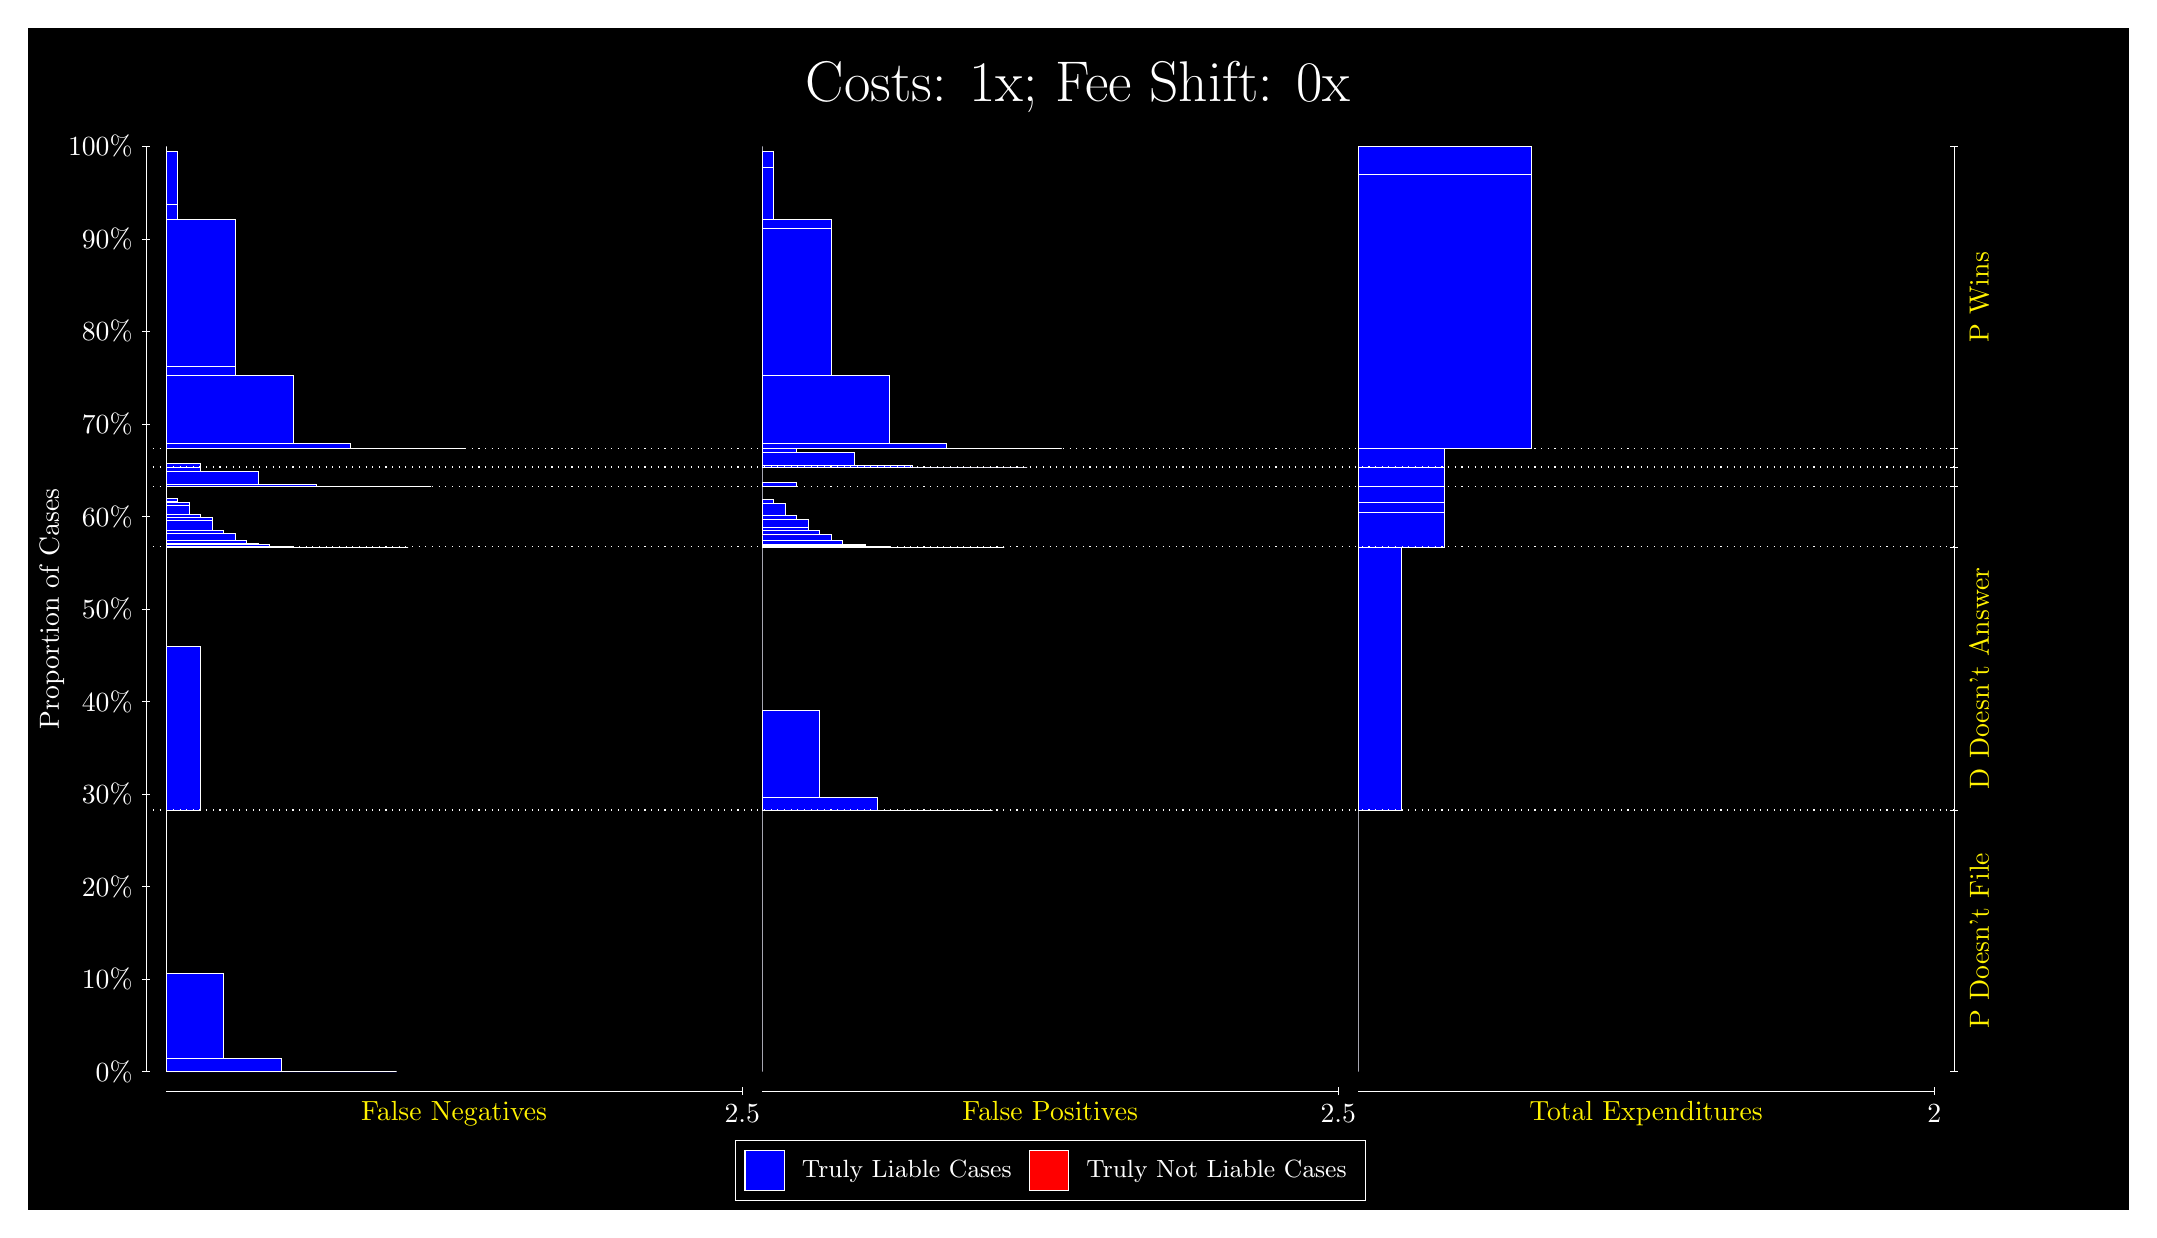
\begin{tikzpicture}
\draw[fill=black] (0,0) rectangle (26.667,15);
\draw[text=white] (0,13.5) rectangle (26.667,15) node[midway] {\huge Costs: 1x; Fee Shift: 0x};
\draw[white, very thin] (1.5,1.75) -- (1.5,13.5);
\node[rotate=90, text=white, anchor=center] at (0.3, 7.625) {Proportion of Cases};
\draw[white, very thin] (1.45,1.75) -- (1.55,1.75);
\node[text=white, anchor=east] at (1.45, 1.75) {0\%};
\draw[white, very thin] (1.45,2.925) -- (1.55,2.925);
\node[text=white, anchor=east] at (1.45, 2.925) {10\%};
\draw[white, very thin] (1.45,4.1) -- (1.55,4.1);
\node[text=white, anchor=east] at (1.45, 4.1) {20\%};
\draw[white, very thin] (1.45,5.275) -- (1.55,5.275);
\node[text=white, anchor=east] at (1.45, 5.275) {30\%};
\draw[white, very thin] (1.45,6.45) -- (1.55,6.45);
\node[text=white, anchor=east] at (1.45, 6.45) {40\%};
\draw[white, very thin] (1.45,7.625) -- (1.55,7.625);
\node[text=white, anchor=east] at (1.45, 7.625) {50\%};
\draw[white, very thin] (1.45,8.8) -- (1.55,8.8);
\node[text=white, anchor=east] at (1.45, 8.8) {60\%};
\draw[white, very thin] (1.45,9.975) -- (1.55,9.975);
\node[text=white, anchor=east] at (1.45, 9.975) {70\%};
\draw[white, very thin] (1.45,11.15) -- (1.55,11.15);
\node[text=white, anchor=east] at (1.45, 11.15) {80\%};
\draw[white, very thin] (1.45,12.325) -- (1.55,12.325);
\node[text=white, anchor=east] at (1.45, 12.325) {90\%};
\draw[white, very thin] (1.45,13.5) -- (1.55,13.5);
\node[text=white, anchor=east] at (1.45, 13.5) {100\%};

\draw[white, very thin] (24.457,1.75) -- (24.457,13.5);
\draw[white, very thin] (24.407,1.75) -- (24.507,1.75);
\node[anchor=west] at (24.407, 1.75) {};
\draw[white, very thin] (24.407,5.0718) -- (24.507,5.0718);
\node[anchor=west] at (24.407, 5.0718) {};
\draw[white, very thin] (24.407,8.4137) -- (24.507,8.4137);
\node[anchor=west] at (24.407, 8.4137) {};
\draw[white, very thin] (24.407,9.1836) -- (24.507,9.1836);
\node[anchor=west] at (24.407, 9.1836) {};
\draw[white, very thin] (24.407,9.4275) -- (24.507,9.4275);
\node[anchor=west] at (24.407, 9.4275) {};
\draw[white, very thin] (24.407,9.6656) -- (24.507,9.6656);
\node[anchor=west] at (24.407, 9.6656) {};
\draw[white, very thin] (24.407,13.5) -- (24.507,13.5);
\node[anchor=west] at (24.407, 13.5) {};

\draw[white, very thin, fill=blue] (1.75,1.75) rectangle (4.6775,1.75);
\draw[white, very thin, fill=blue] (1.75,1.75) rectangle (3.9457,1.7514);
\draw[white, very thin, fill=blue] (1.75,1.7514) rectangle (3.2138,1.9195);
\draw[white, very thin, fill=blue] (1.75,1.9195) rectangle (2.4819,3.0003);
\draw[white, very thin, fill=red] (1.75,3.0003) rectangle (1.75,3.0003);
\draw[white, very thin, fill=blue] (1.75,3.0003) rectangle (1.75,5.0718);
\draw[white, very thin, fill=blue] (1.75,5.0718) rectangle (2.1891,7.1495);
\draw[white, very thin, fill=red] (1.75,7.1495) rectangle (1.75,7.1495);
\draw[white, very thin, fill=blue] (1.75,7.1495) rectangle (1.75,8.4137);
\draw[white, very thin, fill=blue] (1.75,8.4137) rectangle (4.8239,8.4137);
\draw[white, very thin, fill=blue] (1.75,8.4137) rectangle (4.5312,8.4137);
\draw[white, very thin, fill=blue] (1.75,8.4137) rectangle (4.2384,8.4137);
\draw[white, very thin, fill=blue] (1.75,8.4137) rectangle (4.092,8.4137);
\draw[white, very thin, fill=blue] (1.75,8.4137) rectangle (3.9457,8.4137);
\draw[white, very thin, fill=blue] (1.75,8.4137) rectangle (3.7993,8.4137);
\draw[white, very thin, fill=blue] (1.75,8.4137) rectangle (3.6529,8.4137);
\draw[white, very thin, fill=blue] (1.75,8.4137) rectangle (3.5065,8.4138);
\draw[white, very thin, fill=blue] (1.75,8.4138) rectangle (3.3602,8.4267);
\draw[white, very thin, fill=blue] (1.75,8.4267) rectangle (3.2138,8.4268);
\draw[white, very thin, fill=blue] (1.75,8.4268) rectangle (3.0674,8.4416);
\draw[white, very thin, fill=blue] (1.75,8.4416) rectangle (3.0674,8.4493);
\draw[white, very thin, fill=blue] (1.75,8.4493) rectangle (2.921,8.458);
\draw[white, very thin, fill=blue] (1.75,8.458) rectangle (2.7746,8.4909);
\draw[white, very thin, fill=blue] (1.75,8.4909) rectangle (2.6283,8.5017);
\draw[white, very thin, fill=blue] (1.75,8.5017) rectangle (2.6283,8.582);
\draw[white, very thin, fill=blue] (1.75,8.582) rectangle (2.4819,8.6262);
\draw[white, very thin, fill=blue] (1.75,8.6262) rectangle (2.3355,8.7506);
\draw[white, very thin, fill=blue] (1.75,8.7506) rectangle (2.3355,8.7861);
\draw[white, very thin, fill=blue] (1.75,8.7861) rectangle (2.1891,8.8301);
\draw[white, very thin, fill=blue] (1.75,8.8301) rectangle (2.0428,8.9394);
\draw[white, very thin, fill=blue] (1.75,8.9394) rectangle (2.0428,8.9782);
\draw[white, very thin, fill=blue] (1.75,8.9782) rectangle (1.8964,8.9911);
\draw[white, very thin, fill=blue] (1.75,8.9911) rectangle (1.8964,9.0292);
\draw[white, very thin, fill=blue] (1.75,9.0292) rectangle (1.75,9.0292);
\draw[white, very thin, fill=red] (1.75,9.0292) rectangle (1.75,9.0292);
\draw[white, very thin, fill=blue] (1.75,9.0292) rectangle (1.75,9.1836);
\draw[white, very thin, fill=blue] (1.75,9.1836) rectangle (5.1167,9.1836);
\draw[white, very thin, fill=blue] (1.75,9.1836) rectangle (4.3848,9.1837);
\draw[white, very thin, fill=blue] (1.75,9.1837) rectangle (3.6529,9.214);
\draw[white, very thin, fill=blue] (1.75,9.214) rectangle (2.921,9.3741);
\draw[white, very thin, fill=blue] (1.75,9.3741) rectangle (2.1891,9.4275);
\draw[white, very thin, fill=red] (1.75,9.4275) rectangle (1.75,9.4275);
\draw[white, very thin, fill=blue] (1.75,9.4275) rectangle (2.1891,9.481);
\draw[white, very thin, fill=red] (1.75,9.481) rectangle (1.75,9.481);
\draw[white, very thin, fill=blue] (1.75,9.481) rectangle (1.75,9.6656);
\draw[white, very thin, fill=blue] (1.75,9.6656) rectangle (5.5558,9.6656);
\draw[white, very thin, fill=blue] (1.75,9.6656) rectangle (4.8239,9.666);
\draw[white, very thin, fill=blue] (1.75,9.666) rectangle (4.092,9.7302);
\draw[white, very thin, fill=blue] (1.75,9.7302) rectangle (3.3602,10.595);
\draw[white, very thin, fill=blue] (1.75,10.595) rectangle (2.6283,10.703);
\draw[white, very thin, fill=blue] (1.75,10.703) rectangle (2.6283,12.569);
\draw[white, very thin, fill=blue] (1.75,12.569) rectangle (1.8964,12.767);
\draw[white, very thin, fill=blue] (1.75,12.767) rectangle (1.8964,13.435);
\draw[white, very thin, fill=red] (1.75,13.435) rectangle (1.75,13.435);
\draw[white, very thin, fill=blue] (1.75,13.435) rectangle (1.75,13.5);
\draw[white, very thin, fill=red] (9.3189,1.75) rectangle (9.3189,1.75);
\draw[white, very thin, fill=blue] (9.3189,1.75) rectangle (9.3189,5.0718);
\draw[white, very thin, fill=red] (9.3189,5.0718) rectangle (12.246,5.0718);
\draw[white, very thin, fill=blue] (9.3189,5.0718) rectangle (12.246,5.0718);
\draw[white, very thin, fill=blue] (9.3189,5.0718) rectangle (11.515,5.0726);
\draw[white, very thin, fill=blue] (9.3189,5.0726) rectangle (10.783,5.2334);
\draw[white, very thin, fill=blue] (9.3189,5.2334) rectangle (10.051,6.336);
\draw[white, very thin, fill=blue] (9.3189,6.336) rectangle (9.3189,8.4137);
\draw[white, very thin, fill=red] (9.3189,8.4137) rectangle (12.393,8.4137);
\draw[white, very thin, fill=blue] (9.3189,8.4137) rectangle (12.393,8.4137);
\draw[white, very thin, fill=red] (9.3189,8.4137) rectangle (12.1,8.4137);
\draw[white, very thin, fill=blue] (9.3189,8.4137) rectangle (12.1,8.4137);
\draw[white, very thin, fill=red] (9.3189,8.4137) rectangle (11.807,8.4137);
\draw[white, very thin, fill=blue] (9.3189,8.4137) rectangle (11.807,8.4137);
\draw[white, very thin, fill=blue] (9.3189,8.4137) rectangle (11.661,8.4137);
\draw[white, very thin, fill=red] (9.3189,8.4137) rectangle (11.515,8.4137);
\draw[white, very thin, fill=blue] (9.3189,8.4137) rectangle (11.515,8.4137);
\draw[white, very thin, fill=blue] (9.3189,8.4137) rectangle (11.368,8.4137);
\draw[white, very thin, fill=red] (9.3189,8.4137) rectangle (11.222,8.4137);
\draw[white, very thin, fill=blue] (9.3189,8.4137) rectangle (11.222,8.4137);
\draw[white, very thin, fill=blue] (9.3189,8.4137) rectangle (11.075,8.4138);
\draw[white, very thin, fill=red] (9.3189,8.4138) rectangle (10.929,8.4138);
\draw[white, very thin, fill=blue] (9.3189,8.4138) rectangle (10.929,8.4206);
\draw[white, very thin, fill=red] (9.3189,8.4206) rectangle (10.929,8.4206);
\draw[white, very thin, fill=blue] (9.3189,8.4206) rectangle (10.929,8.4206);
\draw[white, very thin, fill=blue] (9.3189,8.4206) rectangle (10.783,8.4207);
\draw[white, very thin, fill=blue] (9.3189,8.4207) rectangle (10.636,8.4314);
\draw[white, very thin, fill=red] (9.3189,8.4314) rectangle (10.636,8.4314);
\draw[white, very thin, fill=blue] (9.3189,8.4314) rectangle (10.636,8.4459);
\draw[white, very thin, fill=blue] (9.3189,8.4459) rectangle (10.49,8.4516);
\draw[white, very thin, fill=red] (9.3189,8.4516) rectangle (10.344,8.4516);
\draw[white, very thin, fill=blue] (9.3189,8.4516) rectangle (10.344,8.4959);
\draw[white, very thin, fill=blue] (9.3189,8.4959) rectangle (10.197,8.5681);
\draw[white, very thin, fill=blue] (9.3189,8.5681) rectangle (10.197,8.5681);
\draw[white, very thin, fill=red] (9.3189,8.5681) rectangle (10.051,8.5681);
\draw[white, very thin, fill=blue] (9.3189,8.5681) rectangle (10.051,8.6191);
\draw[white, very thin, fill=blue] (9.3189,8.6191) rectangle (9.9044,8.6579);
\draw[white, very thin, fill=blue] (9.3189,8.6579) rectangle (9.9044,8.7672);
\draw[white, very thin, fill=blue] (9.3189,8.7672) rectangle (9.758,8.8112);
\draw[white, very thin, fill=blue] (9.3189,8.8112) rectangle (9.6116,8.9711);
\draw[white, very thin, fill=blue] (9.3189,8.9711) rectangle (9.4652,9.0144);
\draw[white, very thin, fill=blue] (9.3189,9.0144) rectangle (9.4652,9.0153);
\draw[white, very thin, fill=blue] (9.3189,9.0153) rectangle (9.3189,9.1836);
\draw[white, very thin, fill=red] (9.3189,9.1836) rectangle (9.758,9.1836);
\draw[white, very thin, fill=blue] (9.3189,9.1836) rectangle (9.758,9.237);
\draw[white, very thin, fill=blue] (9.3189,9.237) rectangle (9.3189,9.4275);
\draw[white, very thin, fill=red] (9.3189,9.4275) rectangle (12.686,9.4275);
\draw[white, very thin, fill=blue] (9.3189,9.4275) rectangle (12.686,9.4275);
\draw[white, very thin, fill=blue] (9.3189,9.4275) rectangle (11.954,9.4275);
\draw[white, very thin, fill=blue] (9.3189,9.4275) rectangle (11.222,9.4554);
\draw[white, very thin, fill=blue] (9.3189,9.4554) rectangle (10.49,9.6121);
\draw[white, very thin, fill=blue] (9.3189,9.6121) rectangle (9.758,9.6656);
\draw[white, very thin, fill=red] (9.3189,9.6656) rectangle (13.125,9.6656);
\draw[white, very thin, fill=blue] (9.3189,9.6656) rectangle (13.125,9.6656);
\draw[white, very thin, fill=red] (9.3189,9.6656) rectangle (12.393,9.6656);
\draw[white, very thin, fill=blue] (9.3189,9.6656) rectangle (12.393,9.6661);
\draw[white, very thin, fill=red] (9.3189,9.6661) rectangle (11.661,9.6661);
\draw[white, very thin, fill=blue] (9.3189,9.6661) rectangle (11.661,9.7309);
\draw[white, very thin, fill=red] (9.3189,9.7309) rectangle (10.929,9.7309);
\draw[white, very thin, fill=blue] (9.3189,9.7309) rectangle (10.929,10.597);
\draw[white, very thin, fill=blue] (9.3189,10.597) rectangle (10.197,12.46);
\draw[white, very thin, fill=red] (9.3189,12.46) rectangle (10.197,12.46);
\draw[white, very thin, fill=blue] (9.3189,12.46) rectangle (10.197,12.57);
\draw[white, very thin, fill=blue] (9.3189,12.57) rectangle (9.4652,13.231);
\draw[white, very thin, fill=blue] (9.3189,13.231) rectangle (9.4652,13.435);
\draw[white, very thin, fill=blue] (9.3189,13.435) rectangle (9.3189,13.5);
\draw[white, very thin, fill=red] (16.888,1.75) rectangle (16.888,1.75);
\draw[white, very thin, fill=blue] (16.888,1.75) rectangle (16.888,5.0718);
\draw[white, very thin, fill=red] (16.888,5.0718) rectangle (17.437,5.0718);
\draw[white, very thin, fill=blue] (16.888,5.0718) rectangle (17.437,8.4137);
\draw[white, very thin, fill=red] (16.888,8.4137) rectangle (17.986,8.4137);
\draw[white, very thin, fill=blue] (16.888,8.4137) rectangle (17.986,8.8513);
\draw[white, very thin, fill=red] (16.888,8.8513) rectangle (17.986,8.8513);
\draw[white, very thin, fill=blue] (16.888,8.8513) rectangle (17.986,8.9825);
\draw[white, very thin, fill=red] (16.888,8.9825) rectangle (17.986,8.9825);
\draw[white, very thin, fill=blue] (16.888,8.9825) rectangle (17.986,9.1836);
\draw[white, very thin, fill=red] (16.888,9.1836) rectangle (17.986,9.1836);
\draw[white, very thin, fill=blue] (16.888,9.1836) rectangle (17.986,9.4275);
\draw[white, very thin, fill=red] (16.888,9.4275) rectangle (17.986,9.4275);
\draw[white, very thin, fill=blue] (16.888,9.4275) rectangle (17.986,9.6656);
\draw[white, very thin, fill=red] (16.888,9.6656) rectangle (19.083,9.6656);
\draw[white, very thin, fill=blue] (16.888,9.6656) rectangle (19.083,13.145);
\draw[white, very thin, fill=red] (16.888,13.145) rectangle (19.083,13.145);
\draw[white, very thin, fill=blue] (16.888,13.145) rectangle (19.083,13.5);
\draw[white, dotted] (1.5,5.0718) -- (24.457,5.0718);
\draw[white, dotted] (1.5,8.4137) -- (24.457,8.4137);
\draw[white, dotted] (1.5,9.1836) -- (24.457,9.1836);
\draw[white, dotted] (1.5,9.4275) -- (24.457,9.4275);
\draw[white, dotted] (1.5,9.6656) -- (24.457,9.6656);
\draw[white, very thin] (1.75,1.5) -- (9.0689,1.5);
\node[text=yellow, anchor=north] at (5.4094, 1.5) {False Negatives};
\draw[white, very thin] (9.0689,1.45) -- (9.0689,1.55);
\node[text=white, anchor=north] at (9.0689, 1.45) {2.5};

\draw[white, very thin] (9.3189,1.5) -- (16.638,1.5);
\node[text=yellow, anchor=north] at (12.978, 1.5) {False Positives};
\draw[white, very thin] (16.638,1.45) -- (16.638,1.55);
\node[text=white, anchor=north] at (16.638, 1.45) {2.5};

\draw[white, very thin] (16.888,1.5) -- (24.207,1.5);
\node[text=yellow, anchor=north] at (20.547, 1.5) {Total Expenditures};
\draw[white, very thin] (24.207,1.45) -- (24.207,1.55);
\node[text=white, anchor=north] at (24.207, 1.45) {2};

\node[text=yellow, centered, rotate=90] at (24.777, 3.4109) {P Doesn't File};
\node[text=yellow, centered, rotate=90] at (24.777, 6.7428) {D Doesn't Answer};



\node[text=yellow, centered, rotate=90] at (24.777, 11.583) {P Wins};

\draw (12.978300999999998,1.5) node[draw=none] (baseCoordinate) {};
\begin{scope}[align=center]
        \matrix[scale=0.5, draw=white, below=0.5cm of baseCoordinate, nodes={draw}, column sep=0.1cm]{
            \node[rectangle, draw, minimum width=0.5cm, minimum height=0.5cm, fill=blue] {}; &
            \node[draw=none, font=\small, text=white] (B) {Truly Liable Cases}; &
            \node[rectangle, draw, minimum width=0.5cm, minimum height=0.5cm, fill=red] {}; &
            \node[draw=none, font=\small, text=white] (B) {Truly Not Liable Cases}; \\
            };
\end{scope}

\end{tikzpicture}
\end{document}